\chapter{Conclusion}
brief of conclusion

\section{Conclusion of Problems}
Tell about solving the problem

\section{Conclusion of Method}
Tell about solving using method

\section{Conclusion of Experiment}
Tell about solving in the experiment

\section{Conclusion of Result}
tell about result for purpose of this research.

\section{Andri Fajar Sunandhar / 1164065}
\subsection{Teori}
\begin{enumerate}
\item Jelaskan kenapa kata-kata harus dilakukan vektorisasi. Dilengkapi dengan ilustrasi atau Gambar
\par Karena mesin hanya mampu membaca data dengan bentuk angka. Berdasarkan hal tersebut maka tentunya diperlukan vektorisasi kata atau bisa disebut dengan mengubah kata menjadi bentuk vektor agar mesin seolah-olah paham apa yang kita maksudkan dan dapat memproses aktifitas/perintah dengan benar. Kata juga harus di vektorisas iuntuk mengetahui presentase kata yang sering muncul dalam setiap kalimatnya, yang berguna untuk menetukan kata kunci. Ilustrasinya bisa dilihat pada gambar berikut  \ref{no1}.
\begin{figure}[ht]
\centerline{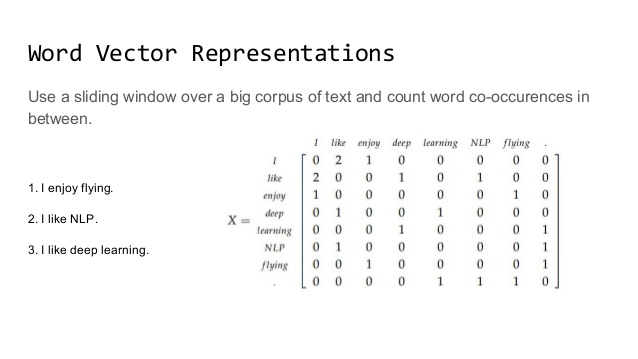
\includegraphics[width=0.5\textwidth]{figures/AFS/no1.jpg}}
\caption{Gambar Vektorisasi Kata.}
\label{no1}
\end{figure}

\item Jelaskan mengapa dimensi dari vektor dataset google bisa sampai 300. Dilengkapi dengan ilustrasi atau Gambar
\par Masing-masing nilai dalam vektor 300 dimensi yang terkait dalam sebua kata "dioptimalkan" dalam  beberapa hal untuk menangkap aspek yang  berbeda dari makna dan penggunaan kata itu.Dengan kata lain masing-masing dari 300 nilai sesuai dengan beberapa fitur abstrak kata. Menghapus kombinasi nilai-nilai ini secara acak akan menghasilkan vektor yang mungkin kurang informasi penting tentang kata tersebut dan mungkin tidak lagi berfungsi sebagai representasi yang baik dari kata itu. Atau singkat cerita mungkin ada lebih dari 3 miliar kata-kata dan kalimat atau data yang tidak mungkin disimpan dalam 1 diemensi vektor makan disimpan menjadi 300 dimensi vektor untuk mengurangi kegagalan memori.  Ilustrasinya bisa dilihat pada gambar berikut   \ref{no2}.
\begin{figure}[ht]
\centerline{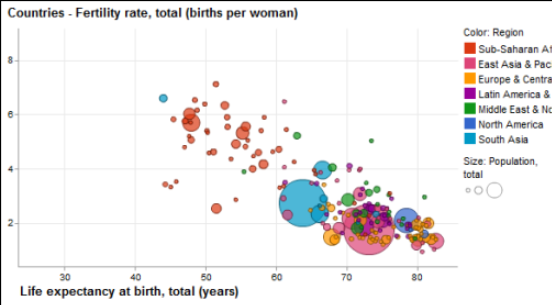
\includegraphics[width=0.5\textwidth]{figures/AFS/no2.png}}
\caption{Gambar Vektorisasi Dataset Google.}
\label{no2}
\end{figure}

\item Jelaskan konsep vektorisasi untuk kata. Dilengkapi dengan ilustrasi atau Gambar
\par Konsep untuk vektorisasi kata sebenarnya sama dengan ketika dilakukan input suatu kata pada mesin pencarian. Kemudian untuk hasilnya akan mengeluarkan ( berupa ) referensi mengenai kata tersebut. Jadi data kata tersebut didapatkan dari hasil pengolahan pada kalimat-kalimat sebelumnya yang telah diolah. Contoh sederhananya pada kalimat berikut ( Please click the alarm icon for more notifications about my channel ), pada kalimat tersebut terdapat konteks yakni channel, kata tersebut akan dijadikan data latih untuk mesin yang akan dipelajari dan diproses. Jadi ketika kita inputkan kta channel, maka mesin akan menampilkan keterkaitannya dengan kata tersebut sehingga akan lebih efisien dan lebih mudah.  Ilustrasinya bisa dilihat pada gambar berikut  \ref{no3}.
\begin{figure}[ht]
\centerline{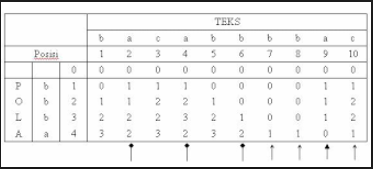
\includegraphics[width=0.5\textwidth]{figures/AFS/no3.png}}
\caption{Gambari Vektorisasi Kata.}
\label{no3}
\end{figure}

\item Jelaskan konesep vektorisasai untuk dokumen. Dilengkapi dengan ilustrasi atau Gambar
\par Vektorisasi Dokumen sebenarnya terbilang sama dengan konsep vektorisasi kata, hanya yang membedakan pada proses awalnya ( pada eksekusi awal ). Untuk vektorisasi dokumen ini, mesin akan membaca semua kalimat yang terdapat pada dokumen tersebut, kemudian kalimat yang terdapat pada dokumen tersebut akan di pecah menjadi kata-kata. Ilustrasinya bisa dilihat pada gambar berikut  \ref{no4}.
\begin{figure}[ht]
\centerline{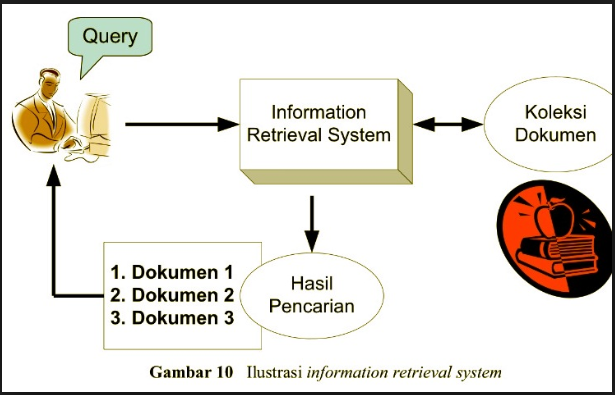
\includegraphics[width=0.5\textwidth]{figures/AFS/no4.png}}
\caption{Gambar Vektorisasi Dokumen.}
\label{no4}
\end{figure}

\item Jelaskan apa mean dan standar deviasi. Dilengkapi dengan ilustrasi atau Gambar
\par Mean adalah teknik penjelasan kelompok yang didasarkan atas nilai rata-rata dari kelompok tersebut. Rata-Rata (mean) ini didapat dengan menjumlahkan data seluruh individu dalam kelompok itu, kemudian dibagi dengan jumlah individu yang ada pada kelompok tersebut. \ref{no5m}
\begin{figure}[ht]
\centerline{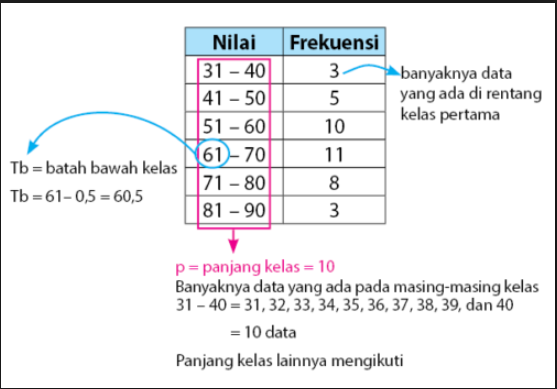
\includegraphics[width=0.5\textwidth]{figures/AFS/no5m.png}}
\caption{Gambar Mean.}
\label{no5m}
\end{figure}

\par Untuk standar deviasi sendiri merupakan sebuah teknik statistik yang digunakan dalam menjelaskan homogenitas kelompok ataupun dapat diartikan dengan nilai statistik dimana dimanfaatkan untuk menentukan bagaimana sebaran data dalam sampel, serta seberapa dekat titik data individu ke mean atau rata-rata nilai sampel yang ada. Ilustrasinya bisa dilihat pada gambar berikut  \ref{no5d}
\begin{figure}[ht]
\centerline{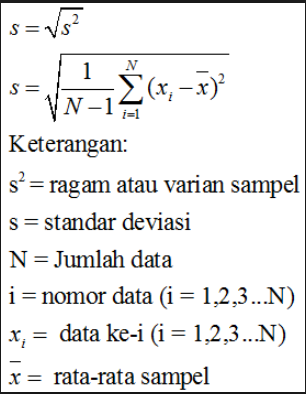
\includegraphics[width=0.5\textwidth]{figures/AFS/no5d.png}}
\caption{Gambar Deviasi.}
\label{no5d}
\end{figure}

\item Jelaskan apa itu skip-gram. Dilengkapi dengan ilustrasi atau Gambar
\par Skip-Gram mencoba memprediksi vektor kata-kata yang ada di konteks diberikan vektor kata tertentu. Skip-Gram membuat sepasang kata target dan konteks sebagai sebuah instance sehingga Skip-Gram cenderung lebih baik ketika ukuran corpus sangat besar.  Ilustrasinya bisa dilihat pada gambar berikut  \ref{no6}.
\begin{figure}[ht]
\centerline{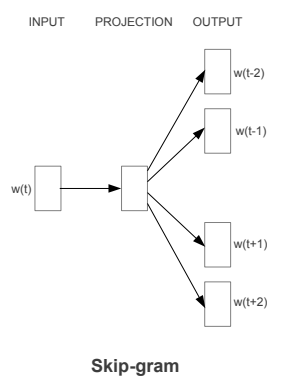
\includegraphics[width=0.5\textwidth]{figures/AFS/no6.png}}
\caption{Gambar Skip-Gram.}
\label{no6}
\end{figure}
\end{enumerate}




\subsection{Praktek Program}
\begin{enumerate}
\item Mencoba dataset google dan menjelaskan vektor dari kata love,faith, fall, sick, clear, shine, bag, car, wash, motor dan cycle. 
\begin{itemize}	
\item Pada gambar \ref{1love} dapat dilihat bahwa vektor memiliki array sebanyak 300 dimensi. Untuk identitas sektor satu adalah 0.10.  
	\begin{figure}[ht]
	\centerline{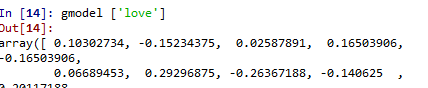
\includegraphics[width=0.5\textwidth]{figures/chapter5/1love.png}}
	\caption{Gambar Vektor Love.}	
	\label{1love}
	\end{figure}


\item Pada gambar \ref{2faith} untuk vektor faith dapat dilihat memliki nilai 0.26 , untuk similaritasnya cukup mendekati vektor love dimana faith dapat dikategorikan dalam satu kategori dengan love.
	\begin{figure}[ht]
	\centerline{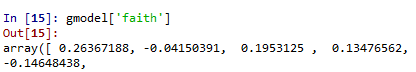
\includegraphics[width=0.5\textwidth]{figures/chapter5/2faith.png}}
	\caption{Gambar vektor faith.}	
	\label{2faith}
	\end{figure}


\item Pada gambar \ref{3fall} Vektor fall hanya memiliki nilai minus yaitu -0.04 , dimana mesin memahami bahwa fall tidak terdapat dalam satu kategori yang sama dengan love dan faith
	\begin{figure}[ht]
	\centerline{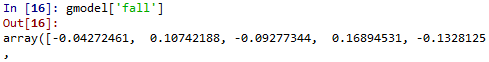
\includegraphics[width=0.5\textwidth]{figures/chapter5/3fall.png}}
	\caption{Gambar vektor fall.}	
	\label{3fall}
	\end{figure}


\item  Pada gambar \ref{4sick} Vektor sick memiliki nilai identitas 1.82 dimana tidak mendekati love, faith maupun fall.
	\begin{figure}[ht]
	\centerline{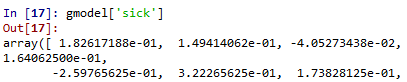
\includegraphics[width=0.5\textwidth]{figures/chapter5/4sick.png}}
	\caption{Gambar vektor sick.}	
	\label{4sick}
	\end{figure}


\item Pada gambar \ref{5clear} Vektor clear memiliki nilai identitas -2,44 dan tidak mendekati nilai dari vektor fall sehingga tidak dapat dijadikan dalam satu kategori
	\begin{figure}[ht]
	\centerline{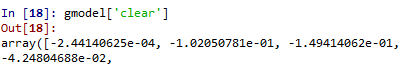
\includegraphics[width=0.5\textwidth]{figures/chapter5/5clear.png}}
	\caption{Gambar vektor clear.}	
	\label{5clear}
	\end{figure}

\item Pada gambar \ref{6shine} Untuk vektor shine -0.12 tidak mendekati vektor manapun.
	\begin{figure}[ht]
	\centerline{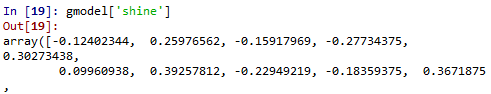
\includegraphics[width=0.5\textwidth]{figures/chapter5/6shine.png}}
	\caption{Gambar vektor shine.}	
	\label{6shine}
	\end{figure}

\item Pada gambar \ref{7bag} Vektor bag memiliki i=nilai identitas -0.03 yang mendekati dengan vektor fall. SEhingga mesin memahami bahwa mungkin saja kedua vektor tersebut berada dalam satu kategori.
	\begin{figure}[ht]
	\centerline{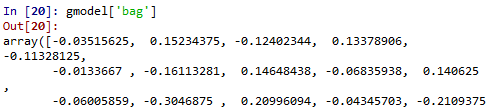
\includegraphics[width=0.5\textwidth]{figures/chapter5/7bag.png}}
	\caption{Gambar vektor bag.}	
	\label{7bag}
	\end{figure}
	

\item Pada gambar \ref{8car} Vektor car nilainya 0.13 mendekati vektor love dan faith sehingga mungkin dapat dikategorikan dalam satu kategori.
	\begin{figure}[ht]
	\centerline{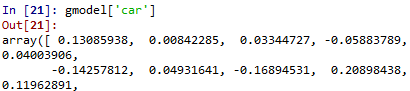
\includegraphics[width=0.5\textwidth]{figures/chapter5/8car.png}}
	\caption{Gambar Vektor car.}	
	\label{8car}
	\end{figure}


\item Pada gambar \ref{9wash} Vektor wash memiliki nilai 9.46 jauh dari vektor vektor lainnya.
	\begin{figure}[ht]
	\centerline{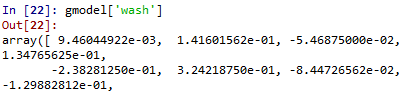
\includegraphics[width=0.5\textwidth]{figures/chapter5/9wash.png}}
	\caption{Gambar Vektor wash.}	
	\label{9wash}
	\end{figure}


\item Pada gambar \ref{10motor} Vektor motor memiliki nilai identitas 5.73 yang bisa mendekati vektor wash. Dapat dikatakan bahwa motor dapat dicuci jika diarti dalam satu kategori yang sama.
	\begin{figure}[ht]
	\centerline{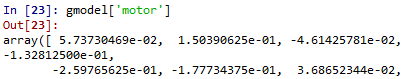
\includegraphics[width=0.5\textwidth]{figures/chapter5/10motor.png}}
	\caption{Gambar vektor motor.}	
	\label{10motor}
	\end{figure}

\item Pada gambar \ref{11cycle} Vektor cycle memiliki nilai identitas 5.73 yang bisa mendekati vektor wash. Dapat dikatakan bahwa motor dapat dicuci jika diarti dalam satu kategori yang sama.
	\begin{figure}[ht]
	\centerline{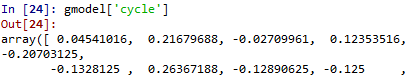
\includegraphics[width=0.5\textwidth]{figures/chapter5/11cycle.png}}
	\caption{Gambar vektor cycle.}	
	\label{11cycle}
	\end{figure}
\end{itemize}

\item Mencoba untuk melakukan perbandingan similirati dari masing-masing kata tersebut. Lihat gambar \ref{12similariti} yang merupakan hasil prediksi similariti
	\begin{figure}[ht]
	\centerline{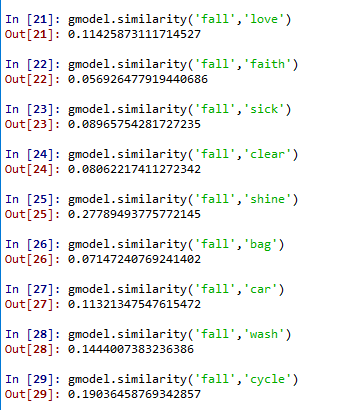
\includegraphics[width=0.5\textwidth]{figures/chapter5/12similariti.png}}
	\caption{Gambar Similariti.}	
	\label{12similariti}
	\end{figure}
	Dapat disimpulkan bahwa:
		\begin{itemize}
		\item Untuk fall dan love hasilnya adalah 11\%
		\item Untuk fall dan faith hasilnya adalah 5\%
		\item Untuk fall dan sick hasilnya adalah 8\%
		\item Untuk fall dan clear hasilnya adalah 8\%
		\item Untuk fall dan shine hasilnya adalah 27\%
		\item Untuk fall dan bag hasilnya adalah 7\%
		\item Untuk fall dan car hasilnya adalah 11\%
		\item Untuk fall dan wash hasilnya adalah 14\%
		\item Untuk fall dan cycle hasilnya adalah 19\%
		
		\end{itemize}
\item Extract Words dan PermuteSentences
	\begin{itemize}
	\item Extract Words : merupakan function untuk menambahkan, menghilangkan atau menghapuskan, hal hal yang tidak penting atau tidakperlu di dalam teks. Dalam contoh gambar \ref{11cycle} ini. menggunakan function extract words untuk menghapus komen dengan python style , mencari data yang diinginkan, dan memberikan spasi pada teks.
		\begin{figure}[ht]
		\centerline{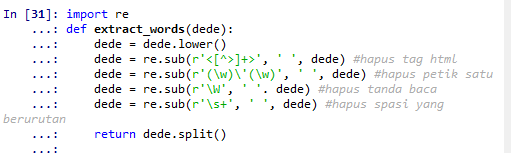
\includegraphics[width=0.5\textwidth]{figures/chapter5/14extract.png}}
		\caption{Gambar Extract Words.}	
		\label{14extract}
		\end{figure}
	\item PermuteSentences : merupakan class yang digunakan unut melakukan pengocokan secara acak pada data yang ada. Digunakan cara ini agar tidak terjadi kelebihan memori pada saat dijalankan. Contoh pada gambar \ref{15permute} yaitu fungsi akan memanggil dede. Yang kemudian mendefinisikan variabel shuffled untuk dede dam melakukan random shuffle yaitu pengocokan acak untuk kata dede.
 		\begin{figure}[ht]
		\centerline{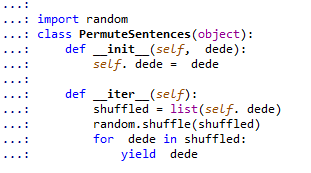
\includegraphics[width=0.5\textwidth]{figures/chapter5/15permute.png}}
		\caption{Gambar PermuteSentences.}	
		\label{15permute}
		\end{figure}
		\end{itemize}
\item Fungsi dari librari gensim TaggedDocument dan Doc2Vec disertai praktek pemakaiannya. Tunjukkan keluarannya dari komputer sendiri dan artikan maksud setiap luaran yang didapatkan.
		\begin{itemize}
		\item Fungsi dari Librari Gensim TaggedDocument dan Doc2Vec :
		\begin{figure}[ht]
		\centerline{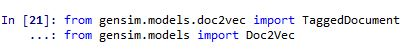
\includegraphics[width=0.5\textwidth]{figures/chapter5/18gensim.jpg}}
		\caption{Gambar librari Gensim}	
		\label{18gensim}
		\end{figure}
		\item Penjelasan pada gambar \ref{18gensim} : yaitu mengimport modul Tagged Document dari model gensim. Sedangkan pada baris kedua import Doc2vec dari model gensim.
		\end{itemize}

\item Cara Menambahkan Data Training
	\begin{itemize}
	\item Penskalaan yaitu dataset ditempatkan sambil mempertimbangkan kumpulan data linier seperti data bank.
	\item  Disintegrasi dan Komposisi: Langkah ini melibatkan pemecahan fitur tertentu untuk membangun data pelatihan yang lebih baik untuk model yang Anda pahami lebih komprehensif.
	\item Komposisi: Ini adalah proses terakhir yang melibatkan penggabungan berbagai fitur menjadi satu fitur untuk mendapatkan data yang lebih akurat atau bermakna.
		\begin{figure}[ht]
		\centerline{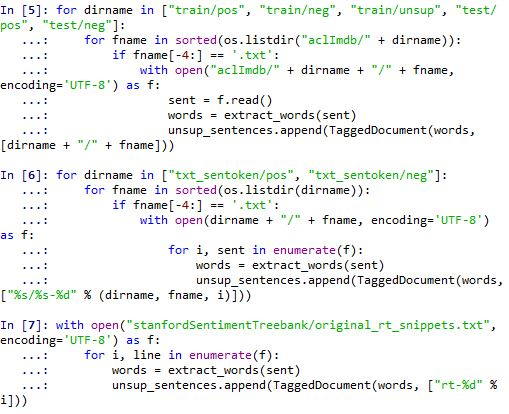
\includegraphics[width=0.5\textwidth]{figures/chapter5/19data.jpg}}
		\caption{Gambar Data Training.}	
		\label{19data}
		\end{figure}
		\item  Penjelasan pada gambar \ref{19data} : Membaca direktori name dari data yang ada di dalam kurung. Pada kodingan di atas ada 3 data. Data pertama yaitu: train/pos,train/neg, train/unsuo, test/pos dan test/neg. Data kedua yaitu:txtsentoken/pos dan txt/sentokenneg. Sedangkan data ke 3 yaitu: standfordSentimentTreeBank/Originalrtsnippes.txt
		\end{itemize}


\item Kenapa Harus Dilakukan Pengocokan dan Pembersih Data
	\par Pengocokan data dilakukan untuk merandom data-data yang ada. Sedangkan pembersihan data dilakukan untuk pengecekan data untuk penetapan dan pemulihan data yang hilang, pengecekan penentapan meliputi pemerikasaan data yang out of range (di luar cakupan) tidak konsisten secara logika, ada nilai-nilai ekstrim, data dengan nilai-nilai tdk terdefinisi, sedangkan pemulihan data yang hilang adalah nilai dari suatu variabel yang tidak diketahui dikarenakan  jawaban responden yang membingungkan.
		\begin{itemize}
		\begin{figure}[ht]
		\centerline{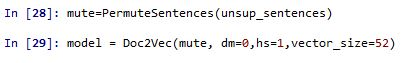
\includegraphics[width=0.5\textwidth]{figures/chapter5/20a.jpg}}
		\caption{Gambar Pengocokan Data.}	
		\label{20a}
		\end{figure}
		\item Penjelasan pada gambar \ref{20a} : yaitu melakukan pengacakan model terhadap data unsupervised learning. 	Dan kemudian baru membuat modelnya setelah dilakukan pengacakan terhadap yang pertama tadi.

		\begin{figure}[ht]
		\centerline{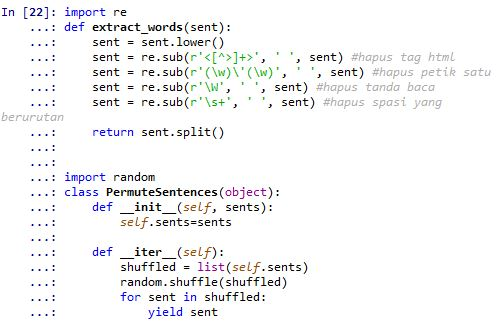
\includegraphics[width=0.5\textwidth]{figures/chapter5/20b.jpg}}
		\caption{Gambar Pembersihan Data.}	
		\label{20b}
		\end{figure}
		\item Penjelasan pada gambar \ref{20b} :  Mengimport Library Re. Kemudian membuat fungsi utuk menghapus tag html dan perkocokan. Dimana di dalam variabel ini ada kodingan untuk menghapus tag html yaitu petik satu, tanda baca dan spasi yang berurutan.
		\end{itemize}

\item Model harus di Save dan Kenapa Temporari Training Harus Dihapus
	\par Karena berfungsi untuk mencegah ram agar tidak lemot dan untuk mengosongkan memori agar sedikit lega atau tidak lemot.
		\begin {itemize}
		\begin{figure}[ht]
		\centerline{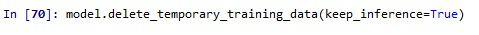
\includegraphics[width=0.5\textwidth]{figures/chapter5/21a.jpeg}}
		\caption{Gambar Temporary Training}	
		\label{21a}
		\end{figure}
		\item Penjelasan pada gambar \ref{21a} : Menghapus Temporary Training Data
		\end {itemize}

\item InferCode
	\par Infercode digunakan untuk menyimpulkan vektor yang berhubungan dengan vektor dokumen baru.
		\begin{itemize}
		\begin{figure}[ht]
		\centerline{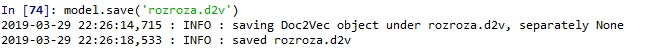
\includegraphics[width=0.5\textwidth]{figures/chapter5/21b.jpeg}}
		\caption{Gambar Infer Code}	
		\label{21a}
		\end{figure}
		\item Penjelasan pada gambar \ref{21a} :  Pada hasil gambar tersebut dapat disimpulkan bahwa kalimat "Belajar Jarkom" menghasilkan outputan berupa array seperti angka-angka di bawah.
		\end{itemize}

\item Cosine Similarity.
		\begin{itemize}
		\begin{figure}[ht]
		\centerline{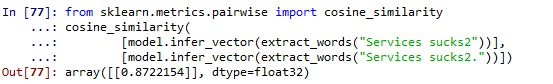
\includegraphics[width=0.5\textwidth]{figures/chapter5/22cosine.jpeg}}
		\caption{Gambar Cosine.}	
		\label{22cosine}
		\end{figure}
		\item  Penjelasan pada gambar \ref{22cosine} : yaitu mengimport cosine similartity dari sklearn metrics pairwise. Dimana cosine similarity berfungsi untuk mengecek kemiripan dari kalimat Services Sucks. Dan akan muncul hasilnya yaitu array.
		\end{itemize}

\item Score Dari Cross Validation
		\begin{itemize}
		\begin{figure}[ht]
		\centerline{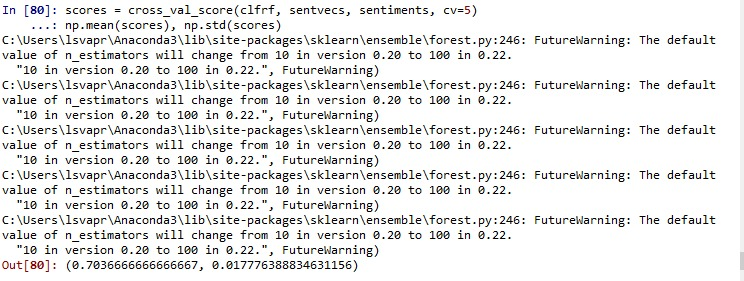
\includegraphics[width=0.5\textwidth]{figures/chapter5/23score.jpeg}}
		\caption{Gambar Score dari cross Validation.}	
		\label{23score}
		\end{figure}
		\item  Penjelasan pada gambar \ref{23score} :  Menghitung model clrf, sentvecs, setiments serta juga meghitung keakuratannya.
		\end{itemize}
\end{enumerate}

\subsection{Penanganan Error}
\begin{enumerate} 
	\item skrinsut error
		\begin{figure}[ht]
		\centering
		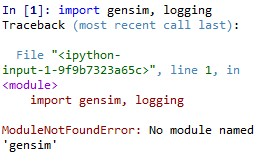
\includegraphics[scale=0.5]{figures/chapter5/16error.jpg}
		\caption{skrinsut error}
		\label{contoh}
		\end{figure}
	\item Tuliskan kode eror dan jenis errornya
		\begin{itemize}
		\item Kode error = ModuleNotFoundError: No module named 'gensim'
		\item Jenis error = Module Not found Error
		\end{itemize}
	\item Solusi pemecahan masalah error
		\par Solusinya adalah dengan mrnginstall modul gensim dengan perintah ...
		\begin{figure}[ht]
		\centering
		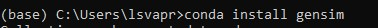
\includegraphics[scale=0.5]{figures/chapter5/17solusi.jpg}
		\caption{Solusi error}
		\label{contoh}
		\end{figure}
	
\end{enumerate}